\documentclass[onecolumn]{article}
\usepackage{graphicx}
\usepackage{float}
\usepackage{hyperref}
\restylefloat{figure}
\begin{document}

\title{Doodles turned into geometric curves}

\author{Arjen Markus}

\maketitle

\section*{Introduction}
I guess everyone draws "doodles" from time to time, meaningless little drawings to while away the time. Such drawings, four are shown in
figure \ref{doodles} below, may feel "geometric", at least, that is how I think about them. You could almost think of an equation or a
parametric representation that would reproduce them and that is exactly what I intend with this note -- construct geometric curves of the
same general shape as the four doodles in the figure.

\begin{figure}[H]
\caption{Four doodles}
\label{doodles}
\begin{center}
\includegraphics[width=0.8\textwidth]{doodles.jpg}
\end{center}
\end{figure}

\section*{The top two doodles: travelling along the horizontal axis}
The first of these, marked "A", is simply the trajectory of a point rotating on a circle while also travelling in the horizontal direction.
So a parametric representation would be:
\begin{eqnarray}
\nonumber x &=& \sin t + At \\
\nonumber y &=& \cos t
\end{eqnarray}

With a particular choice for the constant $A$ you may get the curves in figure~\ref{doodle_a} -- $A = 0.3$. If the constant is smaller, the
loops get closer and overlap. With the constant $A = 1.0$ you get a cycloid.

\begin{figure}[H]
\caption{Doodle A: point on a circle and moving to the right}
\label{doodle_a}
\begin{center}
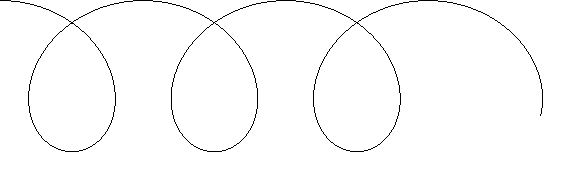
\includegraphics[width=0.8\textwidth]{doodle_a.pdf}
\end{center}
\end{figure}

The second one, "B", might represent a point tracing a figure-eight curve and travelling in the horizontal direction as well. A figure eight
could be a lemniscate\footnote{See \url{https://mathworld.wolfram.com/Lemniscate.html} for more information}, but it could also be a curve
like (the parameter "B" allows us to control the width):
\begin{eqnarray}
\nonumber x &=& B \sin 2t \\
\nonumber y &=& \cos t
\end{eqnarray}

With a component for the horizontal motion you get (figure \ref{doodle_b}):
\begin{eqnarray}
\nonumber x &=& B \sin 2t + At\\
\nonumber y &=& \cos t
\end{eqnarray}

\begin{figure}[H]
\caption{Doodle B: point on a figure-eight curve and moving to the right. Parameter values: $A = 0.2$, $B = -0.6$.}
\label{doodle_b}
\begin{center}
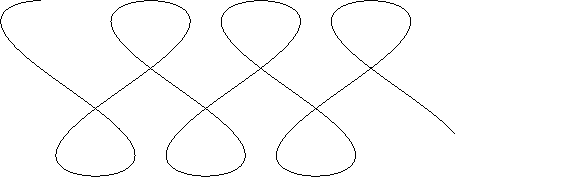
\includegraphics[width=0.8\textwidth]{doodle_b.pdf}
\end{center}
\end{figure}

Note that for the curve to show the intended shape, we need to control the phase via the sign of parameter $B$, otherwise it takes a
shape like in figure \ref{doodle_b2}

\begin{figure}[H]
\caption{Alternative doodle B: point on a figure-eight curve and moving to the right. Parameter values: $A = 0.2$, $B = +0.6$.}
\label{doodle_b2}
\begin{center}
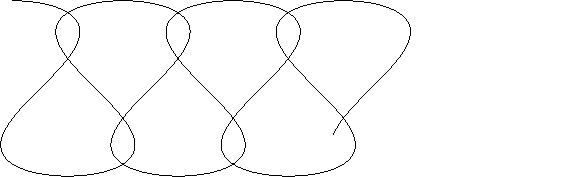
\includegraphics[width=0.8\textwidth]{doodle_b2.pdf}
\end{center}
\end{figure}

\section*{The bottom two doodles: confined curves}
To construct doodle C we need to be a trifle more systematic. By sketching the x- and y-coordinates as a function of a parameter~$t$,
we can get an idea of what the individual equations should be:
\begin{itemize}
\item
If you start at the lowest point and follow the doodle counter-clockwise, then the x-coordinate first increases, then goes to zero
and becomes slightly negative, to follow an opposite course and then to decrease again. This resembles a sine curve with an
additional peak and dip around the value $t = \pi$.
\item
For the y-coordinate we get the following behaviour: from a minimum value it increases to a maximum, then decreases again, but remains above the minimum,
increases again to the same maximum and finally decreases to the same minimum.
\end{itemize}

After some experimentation the result was figure \ref{doodle_c} with equations (the scale factors are a consequence of keeping the curve within a
square of side 2, just like the circle that would result if the second factors are left out):
\begin{eqnarray}
\nonumber x &=& \sin t \cdot (1 + 7.6 \cos t) / 8.6 \\
\nonumber y &=& -\cos t \cdot (1 + 4.6 \cos t) / 5.6
\end{eqnarray}

\begin{figure}[H]
\caption{Doodle C: round curve with a smaller loop at the top.}
\label{doodle_c}
\begin{center}
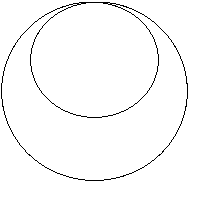
\includegraphics[width=0.5\textwidth]{doodle_c.pdf}
\end{center}
\end{figure}

While experimenting to get the curve in the shape I wanted, I also came across the curve in figure \ref{doodle_c2} with very similar equations:
\begin{eqnarray}
\nonumber x &=& \sin t \cdot (1 + 2.6 \cos t) / 3.6 \\
\nonumber y &=& \cos t \cdot (1 - 2.6 \cos t) / 3.6
\end{eqnarray}

\begin{figure}[H]
\caption{Alternative doodle C: curve resembling a trefoil knot.}
\label{doodle_c2}
\begin{center}
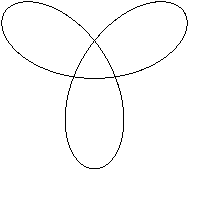
\includegraphics[width=0.5\textwidth]{doodle_c2.pdf}
\end{center}
\end{figure}

Finally, the fourth doodle. This possesses two loops on the side and two cusps on top and bottom. In a similar way as for doodle C we
can analyse the x- and y-coordinates to get an impression of the required functions that will produce this curve. The interesting parts are
the two cusps. They can be represented by a function for $x$ that changes very slowly there and a function for $y$ that has a maximum.
To get the cusp we need $x$ to vary more slowly than $y$. The result is a curve with these parametric equations:
\begin{eqnarray}
\nonumber x &=& \sin ^3 t \\
\nonumber y &=& \cos t + \cos 3t
\end{eqnarray}

The equations are surprisingly simple and elegant, in my opinion.

\begin{figure}[H]
\caption{Doodle D: two loops and two cusps.}
\label{doodle_c}
\begin{center}
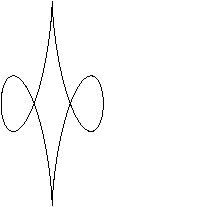
\includegraphics[width=0.5\textwidth]{doodle_d.pdf}
\end{center}
\end{figure}



\end{document}

